\documentclass{article}
\usepackage{tikz}

\begin{document}

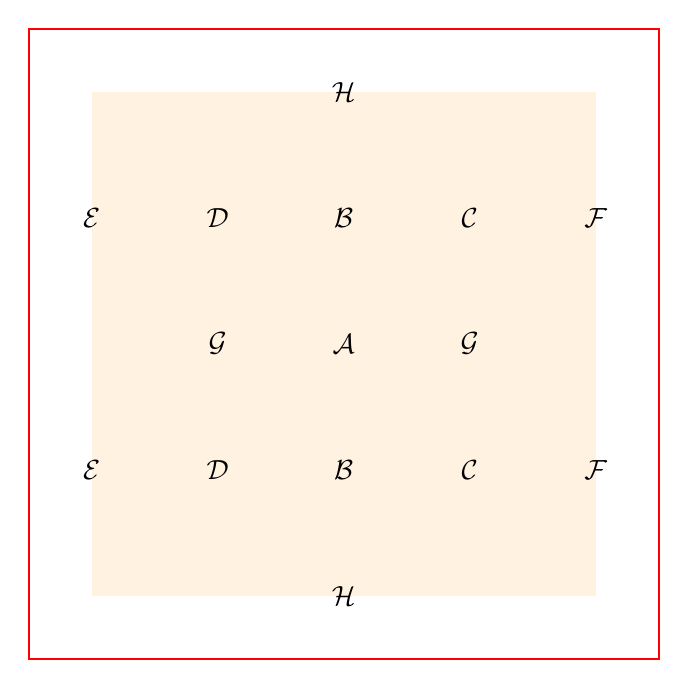
\begin{tikzpicture}[scale=0.8]
    % Define colors
    \definecolor{lightblue}{RGB}{204,238,255}
    \definecolor{lightgreen}{RGB}{211,250,213}
    \definecolor{lightpink}{RGB}{255,204,204}
    \definecolor{lightorange}{RGB}{255,228,196}
    
    % Draw the main rectangle
    \draw[red, thick] (0,0) rectangle (10,10);
    
    % Draw the inner rectangles
    \fill[lightblue] (1,1) rectangle (9,9);
    \fill[lightgreen] (1,1) rectangle (9,9);
    \fill[lightpink] (1,1) rectangle (9,9);
    \fill[lightorange] (1,1) rectangle (9,9);
    
    % Draw the inner shapes
    \fill[lightblue!50] (1,1) rectangle (9,9);
    \fill[lightgreen!50] (1,1) rectangle (9,9);
    \fill[lightpink!50] (1,1) rectangle (9,9);
    \fill[lightorange!50] (1,1) rectangle (9,9);
    
    % Draw the labels
    \node at (5,5) {$\mathcal{A}$};
    \node at (5,7) {$\mathcal{B}$};
    \node at (5,3) {$\mathcal{B}$};
    \node at (7,7) {$\mathcal{C}$};
    \node at (7,3) {$\mathcal{C}$};
    \node at (3,7) {$\mathcal{D}$};
    \node at (3,3) {$\mathcal{D}$};
    \node at (1,7) {$\mathcal{E}$};
    \node at (1,3) {$\mathcal{E}$};
    \node at (9,7) {$\mathcal{F}$};
    \node at (9,3) {$\mathcal{F}$};
    \node at (7,5) {$\mathcal{G}$};
    \node at (3,5) {$\mathcal{G}$};
    \node at (5,1) {$\mathcal{H}$};
    \node at (5,9) {$\mathcal{H}$};
\end{tikzpicture}

\end{document}